\documentclass[a4paper,10pt]{article}
\usepackage[utf8]{inputenc}
\usepackage[T1]{fontenc}
\usepackage[includeheadfoot,hmargin=20mm,vmargin=16mm]{geometry}
\usepackage{times}
\usepackage{booktabs}
\usepackage[small]{titlesec}
\usepackage{enumitem}
\usepackage{amsmath}
\usepackage{amsthm}
\usepackage{mathptmx}
\usepackage{tikz}
\usetikzlibrary{shapes,arrows,decorations.pathreplacing}
\usepackage{xifthen}
\frenchspacing
\setlist{nosep}
\renewcommand{\ttdefault}{cmtt}
\author{Thor Kristoffersen}
\date{September 23, 2020}
\title{The Immortal Virtual Machine\\Instruction Set Architecture\\
  %
  \vspace{1ex}
  \large VirtuMa Solution 3.3 Part a}
\newcommand{\num}[1]{\texttt{#1}}
\newcommand{\hex}[1]{\num{#1}}
%\newcommand{\bin}[1]{\num{#1}_{\textup{\tiny 2}}}
\newcommand{\MEM}[1]{\ifthenelse{\equal{#1}{}}{M}{M[#1]}}
\newcommand{\PC}{PC}
\newcommand{\SP}{SP}
\newcommand{\TERM}{T}
\newcommand{\F}{\bin{0}}
\newcommand{\T}{\bin{1}}
\newcommand{\octno}[2]{#1.\mathrm{octet}[#2]}
\newcommand{\bitno}[2]{#1.\mathrm{bit}[#2]}
\newcommand{\range}[2]{\{#1,\ldots,#2\}}
\newcommand{\width}[2]{(#1)#2}
\newcommand{\set}[2]{#1\;:=\;#2}
\newcommand{\Var}[2]{\mathbf{var}\;#1\;:=\;#2\;}
\newcommand{\dotimes}[4]{\mathbf{for}\;#1\;\mathbf{in}\;#2\ldots#3\;\mathbf{do}\;#4}
\newcommand{\return}[1]{\mathbf{return} \; #1}
\newcommand{\Put}[3]{\mathrm{store}(#1,\;#2,\;#3)}
\newcommand{\Get}[2]{\mathrm{load}(#1,\;#2)}
\newcommand{\Push}[1]{\mathrm{push}(#1)}
\newcommand{\Pop}{\mathrm{pop}()}
\newcommand{\Fetch}[1]{\mathrm{fetch}(#1)}
\newcommand{\PutByte}[1]{\mathrm{putbyte}(#1)}
\newcommand{\PutChar}[1]{\mathrm{putchar}(#1)}
\newcommand{\AddSample}[1]{\mathrm{addsample}(#1)}
\newcommand{\SetPixel}[1]{\mathrm{setpixel}(#1)}
\newcommand{\NewFrame}[1]{\mathrm{newframe}(#1)}
\newcommand{\ReadPixel}[1]{\mathrm{readpixel}(#1)}
\newcommand{\ReadFrame}[1]{\mathrm{readframe}(#1)}
\newcommand{\proc}[1]{\textsc{#1}}
\DeclareMathOperator{\Mod}{mod}
\DeclareMathOperator{\Add}{add}
\DeclareMathOperator{\Mul}{mul}
\DeclareMathOperator{\Div}{div}
\DeclareMathOperator{\Rem}{rem}
\DeclareMathOperator{\BinPow}{pow2}
\DeclareMathOperator{\BitAnd}{and}
\DeclareMathOperator{\BitOr}{or}
\DeclareMathOperator{\BitNot}{not}
\DeclareMathOperator{\BitXor}{xor}
\DeclareMathOperator{\IfThEl}{if}
\newcommand{\modulo}[2]{#1 \Mod #2}
\newcommand{\intdiv}[2]{#1 \Div #2}
\newcommand{\conj}{\wedge}
\newcommand{\inc}[2]{\set{#1}{#1 + #2}}
\newcommand{\dec}[2]{\set{#1}{#1 - #2}}
\newcommand{\comment}[1]{\begin{quote}[\textit{#1}]\end{quote}}
\newcommand{\deviceio}[1]{$\langle$#1$\rangle$}
\newcommand{\op}[3]{\ifthenelse{\equal{#1}{m}}{\texttt{#2}}{$#3$}}
\theoremstyle{definition}
\newtheorem{definition}{Definition}
\newcommand{\memspace}{\qquad}
\newcommand{\EXIT}      [1]{\op{#1}{EXIT}       {\hex{00}}}
\newcommand{\NOP}       [1]{\op{#1}{NOP}        {\hex{01}}}
\newcommand{\JUMP}      [1]{\op{#1}{JUMP}       {\hex{02}}}
\newcommand{\JZFWD}     [1]{\op{#1}{JZ\_FWD}    {\hex{03}}}
\newcommand{\JZBACK}    [1]{\op{#1}{JZ\_BACK}   {\hex{04}}}
\newcommand{\SETSP}     [1]{\op{#1}{SET\_SP}    {\hex{05}}}
\newcommand{\GETPC}     [1]{\op{#1}{GET\_PC}    {\hex{06}}}
\newcommand{\GETSP}     [1]{\op{#1}{GET\_SP}    {\hex{07}}}
\newcommand{\PUSHZ}     [1]{\op{#1}{PUSH0}      {\hex{08}}}
\newcommand{\PUSHB}     [1]{\op{#1}{PUSH1}      {\hex{09}}}
\newcommand{\PUSHS}     [1]{\op{#1}{PUSH2}      {\hex{0A}}}
\newcommand{\PUSHI}     [1]{\op{#1}{PUSH4}      {\hex{0B}}}
\newcommand{\PUSHL}     [1]{\op{#1}{PUSH8}      {\hex{0C}}}
\newcommand{\LOADB}     [1]{\op{#1}{LOAD1}      {\hex{10}}}
\newcommand{\LOADS}     [1]{\op{#1}{LOAD2}      {\hex{11}}}
\newcommand{\LOADI}     [1]{\op{#1}{LOAD4}      {\hex{12}}}
\newcommand{\LOADL}     [1]{\op{#1}{LOAD8}      {\hex{13}}}
\newcommand{\STOREB}    [1]{\op{#1}{STORE1}     {\hex{14}}}
\newcommand{\STORES}    [1]{\op{#1}{STORE2}     {\hex{15}}}
\newcommand{\STOREI}    [1]{\op{#1}{STORE4}     {\hex{16}}}
\newcommand{\STOREL}    [1]{\op{#1}{STORE8}     {\hex{17}}}
\newcommand{\ADD}       [1]{\op{#1}{ADD}        {\hex{20}}}
\newcommand{\MULT}      [1]{\op{#1}{MULT}       {\hex{21}}}
\newcommand{\DIV}       [1]{\op{#1}{DIV}        {\hex{22}}}
\newcommand{\REM}       [1]{\op{#1}{REM}        {\hex{23}}}
\newcommand{\LT}        [1]{\op{#1}{LT}         {\hex{24}}}
\newcommand{\AND}       [1]{\op{#1}{AND}        {\hex{28}}}
\newcommand{\OR}        [1]{\op{#1}{OR}         {\hex{29}}}
\newcommand{\NOT}       [1]{\op{#1}{NOT}        {\hex{2A}}}
\newcommand{\XOR}       [1]{\op{#1}{XOR}        {\hex{2B}}}
\newcommand{\POW}       [1]{\op{#1}{POW2}       {\hex{2C}}}
\newcommand{\PUTBYTE}   [1]{\op{#1}{PUT\_BYTE}  {\hex{F9}}}
\newcommand{\PUTCHAR}   [1]{\op{#1}{PUT\_CHAR}  {\hex{FA}}}
\newcommand{\ADDSAMPLE} [1]{\op{#1}{ADD\_SAMPLE}{\hex{FB}}}
\newcommand{\SETPIXEL}  [1]{\op{#1}{SET\_PIXEL} {\hex{FC}}}
\newcommand{\NEWFRAME}  [1]{\op{#1}{NEW\_FRAME} {\hex{FD}}}
\newcommand{\READPIXEL} [1]{\op{#1}{READ\_PIXEL}{\hex{FE}}}
\newcommand{\READFRAME} [1]{\op{#1}{READ\_FRAME}{\hex{FF}}}

\newlist{stepnumbers}{enumerate}{2}
\setlist[stepnumbers]{label=\textbf{\arabic*},labelsep=0.7em}
\newlist{stepletters}{enumerate}{1}
\setlist[stepletters]{label=\textbf{\alph*}}

\begin{document}

\maketitle

\noindent
The remainder of this document is a semi-formal specification of the Immortal Virtual Machine, written in a style more or less similar to a processor data sheet.

\thispagestyle{empty}
\newpage

~
\thispagestyle{empty}
\newpage
\setcounter{page}{1}

\begin{center}
  \Large{Immortal Virtual Machine\\Instruction Set Architecture}
\end{center}
\vspace{1em}

\section{Programming Model}
\label{sec:programming-model}

The IVM is a pure stack-based machine: it has a program counter and a stack pointer, but no general-purpose registers.
The programming model consists of the following elements:
\begin{itemize}
\item \emph{Memory}:
  An array of 8-bit locations, $\MEM{A..A+N-1}$, where $0 \le A < 2^{64}$ and $0 < N \le 2^{64}$.
\item \emph{Program Counter}:
  A 64-bit register, $\PC$, that points to the next instruction to be fetched or to any immediate operands of an instruction.
  The initial value of $\PC$ is $A$.
\item \emph{Stack Pointer}:
  A 64-bit register, $\SP$, that points to the top of the stack, which is the memory region from $\MEM{\SP}$ to $\MEM{M+N-1}$, inclusive.
  The initial value of $\SP$ is $\modulo{(M+N)}{2^{64}}$.
\item \emph{Terminate Flag}:
  A 1-bit flag, $\TERM$, that is set to $1$ when the machine has terminated.
  The initial value of $\TERM$ is $0$.
\end{itemize}
These elements are shown graphically in the following figure.
\begin{trivlist}
\item\centering
  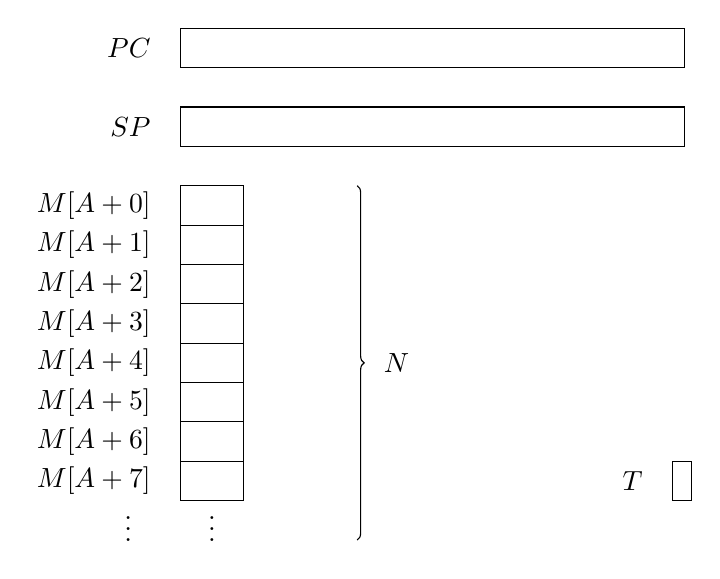
\begin{tikzpicture}[scale=0.5]
    \foreach \y in {0,...,7}
    {
      \draw (0, 7-\y) node[anchor=east] {$\MEM{A+\y}$};
      \draw (0.5, \y) node[anchor=west,minimum width=8mm,minimum height=5mm,draw] {};
    }
    \draw (0, -1) node[anchor=east,minimum width=8mm] {$\vdots$};
    \draw (0.5, -1) node[anchor=west,minimum width=8mm] {$\vdots$};
    \draw (0, 11) node[anchor=east] {$\PC{}$};
    \draw (0, 9) node[anchor=east] {$\SP{}$};
    \draw (12.5, 0) node[anchor=east] {$\TERM{}$};
    \draw (0.5, 11) node[anchor=west,minimum width=64mm,minimum height=5mm,draw] {};
    \draw (0.5, 9) node[anchor=west,minimum width=64mm,minimum height=5mm,draw] {};
    \draw (13, 0) node[anchor=west,minimum width=1mm,minimum height=5mm,draw] {};
    \draw[decorate,decoration=brace] (5,7.5) -- (5,-1.5);
    \draw (6,3) node {$N$};
  \end{tikzpicture}
\end{trivlist}

\section{Basic Definitions}
\label{sec:notation}

\begin{definition}[Floor]
  $\left \lfloor x \right \rfloor$ is the unique integer such that $\left \lfloor x \right \rfloor \le x < (\left \lfloor x \right \rfloor + 1)$.
\end{definition}

\begin{definition}[Integer division]
  \[ \intdiv{x}{y} = \left \lfloor \frac{x}{y} \right \rfloor \]
\end{definition}

\begin{definition}[Modulo]
  \[ \modulo{x}{y} = x - y \left \lfloor \frac{x}{y} \right \rfloor, \quad y > 0 \]
\end{definition}

\begin{definition}[Bit value]
For any integer value, $x$, the notation $\bitno{x}{i}$ refers to the value of bit $i$ in $x$.
\end{definition}

\begin{definition}[Octet value]
For any integer value, $x$, the notation $\octno{x}{i}$ refers to the integer made up of the bit sequence from $\bitno{x}{8i+7}$ to $\bitno{x}{8i}$, inclusive.
\end{definition}

\section{Basic Functions}
\label{sec:function-definitions}

The following functions are needed by some instructions.
For each function, its arguments and its result are all 64-bit integer values, except where otherwise noted.

\begin{definition}[Conditional]
  \[ \IfThEl(e, c, a) = \left\{
      \begin{array}{@{}ll@{}}
        c & \mathrm{if} \; e \; \mathrm{is} \; \mathrm{true} \\
        a & \mathrm{otherwise}
      \end{array}
    \right. \]
\end{definition}

\begin{definition}[Addition]
  \[ \Add(x, y) = \modulo{(x + y)}{2^{64}} \]
\end{definition}

\begin{definition}[Multiplication]
  \[ \Mul(x, y) = \modulo{(x y)}{2^{64}} \]
\end{definition}

\begin{definition}[Integer division]
  \[ \Div(x, y) = 
    \left\{
      \begin{array}{@{}ll@{}}
        q \mid x = qy + r \wedge 0 \leq r < y & \mathrm{if} \; x > 0 \wedge y > 0 \\
        0 & \textrm{otherwise}
      \end{array}
    \right. \]
\end{definition}

\begin{definition}[Integer remainder]
  \[ \Div(x, y) = 
    \left\{
      \begin{array}{@{}ll@{}}
        r \mid x = qy + r \wedge 0 \leq r < y & \mathrm{if} \; x > 0 \wedge y > 0 \\
        0 & \textrm{otherwise}
      \end{array}
    \right. \]
\end{definition}

\begin{definition}[Binary power]
  \[ \BinPow(x) = 
    \left\{
      \begin{array}{@{}ll@{}}
        2^x & \mathrm{if} \; x < 64 \\
        0   & \textrm{otherwise}
      \end{array}
    \right. \]
\end{definition}

\begin{definition}[Bitwise boolean ``and'']
  \[ \BitAnd(x, y) = z \mid  
    \forall i \in \range{0}{63} \mid \bitno{z}{i} = \left\{
      \begin{array}{@{}ll@{}}
        1 & \mathrm{if} \; \bitno{x}{i} = 1 \wedge \bitno{y}{i} = 1 \\
        0 & \mathrm{otherwise}
      \end{array}
    \right. \]
\end{definition}

\begin{definition}[Bitwise boolean ``or'']
  \[ \BitOr(x, y) = z \mid  
    \forall i \in \range{0}{63} \mid \bitno{z}{i} = \left\{
      \begin{array}{@{}ll@{}}
        1 & \mathrm{if} \; \bitno{x}{i} = 1 \vee \bitno{y}{i} = 1 \\
        0 & \mathrm{otherwise}
      \end{array}
    \right. \]
\end{definition}

\begin{definition}[Bitwise boolean ``not'']
  \[ \BitNot(x) = z \mid  
    \forall i \in \range{0}{63} \mid \bitno{z}{i} = \left\{
      \begin{array}{@{}ll@{}}
        1 & \mathrm{if} \; \bitno{x}{i} = 0 \\
        0 & \mathrm{otherwise}
      \end{array}
    \right. \]
\end{definition}

\begin{definition}[Bitwise boolean ``exclusive or'']
  \[ \BitXor(x, y) = z \mid  
    \forall i \in \range{0}{63} \mid \bitno{z}{i} = \left\{
      \begin{array}{@{}ll@{}}
        1 & \mathrm{if} \; \bitno{x}{i} \neq \bitno{y}{i} \\
        0 & \mathrm{otherwise}
      \end{array}
    \right. \]
\end{definition}

\section{Memory Access Procedures}

Five basic procedures for memory access are used as building blocks for the instructions.

\subsection{Pseudocode Elements}

We introduce the following pseudocode elements to describe the procedures in this section.
\begin{itemize}
\item $\set{x}{v}$\\Assign $x$ the value $v$.
\item $\Var{x}{v}$\\Declare variable $x$, assigning it the value of $v$.
\item $\dotimes{i}{m}{n}{S(i)}$\\Evaluate $S(i)$ $n-m$ times, with $i$ successively bound to every integer in the range $\range{m}{n-1}$.
\item $\return{v}$\\Return the value of $v$.
\end{itemize}

\subsection{General Memory Access Operations}

There are two basic procedures for general memory access that instructions can use to store integers to or load integers from a given memory address.
The memory is 8 bits wide, and integers can be 8, 16, 32, or 64 bits wide, so they are stored from the given memory address in little-endian format. 
An 8-bit integer is trivially mapped to the specified memory address.

The procedure $\Put{n}{a}{x}$ stores an integer, $x$, as $n$ octets starting at memory address $a$.
It is defined in pseudocode as follows:
\begin{equation}
  \Put{n}{a}{x} \; \equiv \; \dotimes{i}{0}{n}{\set{\MEM{a + i}}{\octno{x}{i}}}
\end{equation}

The procedure $\Get{n}{a}$ returns an integer loaded from $n$ octets starting at memory address $a$.
It is defined in pseudocode as follows:
\begin{equation}
  \begin{split}
  \Get{n}{a} \; \equiv \; & \Var{x}{0} \\
  & \dotimes{i}{0}{n}{\set{\octno{x}{i}}{\MEM{a + i}}} \\
  & \return{x}
  \end{split}
\end{equation}

\subsection{Stack Operations}

The stack operations are defined in terms of the general memory access operations, using the stack pointer as the memory address.
All stack operations work on 8 octets at a time, so arguments and results are assumed to be 64-bit integers.
For this reason the stack operations also decrement and increment the stack pointer in multiples of 8.

The procedure $\Push{x}$ pushes an integer, $x$, on the stack.
It is defined in pseudocode as follows:
\begin{equation}
  \begin{split}
    \Push{x} \; \equiv \; & \set{\SP}{\modulo{(\SP-8)}{2^{64}}} \\
                       & \Put{8}{\SP}{x}
  \end{split}
\end{equation}

The procedure $\Pop{}$ returns an integer popped off the stack.
It is defined in pseudocode as follows:
\begin{equation}
  \begin{split}
    \Pop{} \; \equiv \; & \Var{x}{\Get{8}{\SP}} \\
    & \set{\SP}{\modulo{(\SP+8)}{2^{64}}} \\
    & \return{x}
  \end{split}
\end{equation}

\subsection{Fetch Operation}

The procedure $\Fetch{n}$ fetches $n$ octets relative to the program counter, incrementing it by the same number.
It is used both to fetch instructions and to fetch immediate operands.

\begin{equation}
  \begin{split}
    \Fetch{n} \equiv \; & \Var{x}{\Get{n}{\PC}} \\
    & \set{\PC}{\modulo{(\PC+n)}{2^{64}}} \\
    & \return{x}
  \end{split}
\end{equation}

\section{Device Access Procedures}

This section describes the procedures for device access.
Since the devices interface the machine with the real world, the semantics can be described only informally.

\subsection{Image Input}
\label{sec:image-input}
The \emph{Image Input} device allows the machine to consume an image as a two-dimensional array of points of light intensity values.
The following figure shows an example of such an array, consisting of 32 sampling points arranged in 8 columns and 4 rows.
\begin{center}
  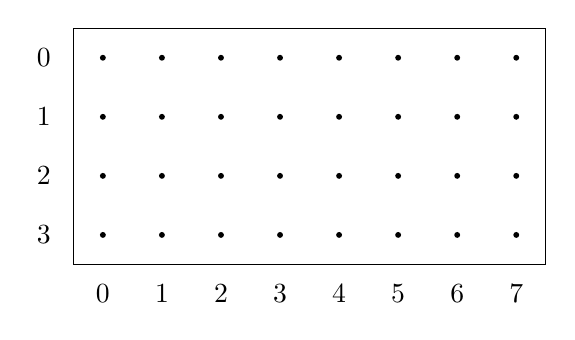
\begin{tikzpicture}[scale=0.75]
    \foreach \x in {0,...,7}
    \foreach \y in {0,...,3}
    {
      \fill (\x,\y) circle [radius=0.5mm,fill=black,draw] {};
    }
    \foreach \x in {0,...,7} \draw (\x, -1) node {\x};
    \foreach \y in {0,...,3} \draw (-1, 3 - \y) node {\y};
    \draw (-0.5,-0.5) -- (7.5,-0.5) -- (7.5,3.5) -- (-0.5,3.5) -- cycle;
  \end{tikzpicture}
\end{center}
As shown, both columns and rows are numbered consecutively, starting at 0.
The spacing between the sampling points must be uniform in both horizontal and vertical directions, and an anti-aliasing filter must be employed to limit the bandwidth of the image to satisfy the Nyquist-Shannon sampling theorem.

Each picture element detects the intensity of light transmitted or reflected at a sampling point in that particular position of the image, represented as one of 256 intensity levels, from 0 (minimum intensity) to 255 (maximum intensity).
Values between 0 and 255 represent intermediate intensities between these extremes.

\begin{definition}[Read frame]
  The $\ReadFrame{}$ operation reads a new frame and returns the number of columns, $c$, and the number of rows $r$.
  \[ (c, r) = \ReadFrame{} \]
\end{definition}

\begin{definition}[Read pixel]
  The $\ReadPixel{}$ operation returns the intensity, $z$, of the point at column $x$ and row $y$.
  \[ z = \ReadPixel{x, y} \]
\end{definition}

\subsection{Image Output}
\label{sec:image-output}

The \emph{Image Output} device allows the machine to produce an image represented as a two-dimensional array of points of color space values.
Moving images can be produced as a sequence of images.

\begin{definition}[New frame]
  The $\NewFrame{}$ operation finishes and renders the frame constructed so far, and it sets the width of the next frame to $w$, the height to $h$, and the sample rate to $r$.
  \[ \NewFrame{w, h, r} \]
\end{definition}

\begin{definition}[Set pixel]
  The $\SetPixel{}$ operation sets the red value to $r$, the green value to $g$, and the blue value to $b$ for the pixel at column $x$ and row $y$.
  \[ \SetPixel{x, y, r, g, b} \]
\end{definition}

\subsection{Audio Output}
\label{sec:audio-output}

The \emph{Audio Output} device allows the machine to produce a two-channel audio signal encoded digitally using Linear Pulse Code Modulation.
The device must create an audio signal passing through a series of magnitude values specified by the program.
The bandwith of this audio signal must be less than half of the sampling frequency.
Each channel value is in the range $\range{0}{2^{16}-1}$.

\begin{definition}[Add sample]
  The $\AddSample{}$ operation sets the audio signal magnitude of the left channel to $l$ and the one of the right channel to $r$.
\[ \AddSample{l, r} \]
\end{definition}

\subsection{Text Output}
\label{sec:text-output}

The \emph{Text Output} device allows the machine to produce a stream of text.

\begin{definition}[Put character]
  The $\PutChar{}$ operation produces the character with Unicode code point $c$.
  \[ \PutChar{c} \]
\end{definition}

\subsection{Octet Output}
\label{sec:octet-output}

The \emph{Text Output} device allows the machine to produce a stream of 8-bit numbers.

\begin{definition}[Put byte]
  The $\PutByte{}$ operation produces the octet $x$.
  \[ \PutByte{x} \]
\end{definition}

%\newpage

\section{Instruction Semantics}
\label{sec:instruction-semantics}

The following table summarizes the instruction semantics.
\begin{trivlist}
\item 
  \begin{tabular}{@{}lllllll@{}}
    Hex           & Mnemonic      & Comment                  & Immediate      & Pop         & Explicit effects                & Push                   \\
    \hline
    \EXIT{c}      & \EXIT{m}      & Stop execution           & --             & --          & $\set{\TERM}{1}$                  & --                     \\
    \NOP{c}       & \NOP{m}       & No operation             & --             & --          & --                                & --                     \\
    \JUMP{c}      & \JUMP{m}      & Jump to address          & --             & $a$         & $\set{\PC}{a}$                    & --                     \\
    \JZFWD{c}     & \JZFWD{m}     & Jump forward on zero     & $\width{1}{d}$ & $x$         & $\inc{\PC}{\IfThEl(x=0, d, 0)}$   & --                     \\
    \JZBACK{c}    & \JZBACK{m}    & Jump backward on zero    & $\width{1}{d}$ & $x$         & $\dec{\PC}{\IfThEl(x=0, d+1, 0)}$ & --                     \\
    \SETSP{c}     & \SETSP{m}     & Set stack pointer        & --             & $a$         & $\set{\SP}{a}$                    & --                     \\
    \GETPC{c}     & \GETPC{m}     & Get program counter      & --             & --          & --                                & $\PC$                  \\
    \GETSP{c}     & \GETSP{m}     & Get stack pointer        & --             & --          & --                                & $\SP$                  \\
    \PUSHZ{c}     & \PUSHZ{m}     & Push literal zero        & --             & --          & --                                & $0$                    \\
    \PUSHB{c}     & \PUSHB{m}     & Push 1 immediate octet   & $\width{1}{x}$ & --          & --                                & $x$                    \\
    \PUSHS{c}     & \PUSHS{m}     & Push 2 immediate octets  & $\width{2}{x}$ & --          & --                                & $x$                    \\
    \PUSHI{c}     & \PUSHI{m}     & Push 4 immediate octets  & $\width{4}{x}$ & --          & --                                & $x$                    \\
    \PUSHL{c}     & \PUSHL{m}     & Push 8 immediate octets  & $\width{8}{x}$ & --          & --                                & $x$                    \\
    \LOADB{c}     & \LOADB{m}     & Load 1 memory octet      & --             & $a$         & --                                & $\Get{1}{a}$           \\
    \LOADS{c}     & \LOADS{m}     & Load 2 memory octets     & --             & $a$         & --                                & $\Get{2}{a}$           \\
    \LOADI{c}     & \LOADI{m}     & Load 4 memory octets     & --             & $a$         & --                                & $\Get{4}{a}$           \\
    \LOADL{c}     & \LOADL{m}     & Load 8 memory octets     & --             & $a$         & --                                & $\Get{8}{a}$           \\
    \STOREB{c}    & \STOREB{m}    & Store 1 memory octet     & --             & $a,x$       & $\Put{1}{a}{x}$                   & --                     \\
    \STORES{c}    & \STORES{m}    & Store 2 memory octets    & --             & $a,x$       & $\Put{2}{a}{x}$                   & --                     \\
    \STOREI{c}    & \STOREI{m}    & Store 4 memory octets    & --             & $a,x$       & $\Put{4}{a}{x}$                   & --                     \\
    \STOREL{c}    & \STOREL{m}    & Store 8 memory octets    & --             & $a,x$       & $\Put{8}{a}{x}$                   & --                     \\
    \ADD{c}       & \ADD{m}       & Add                      & --             & $y,x$       & --                                & $\Add(x, y)$           \\
    \MULT{c}      & \MULT{m}      & Multiply                 & --             & $y,x$       & --                                & $\Mul(x, y)$           \\
    \DIV{c}       & \DIV{m}       & Divide                   & --             & $y,x$       & --                                & $\Div(x, y)$           \\
    \REM{c}       & \REM{m}       & Find remainder           & --             & $y,x$       & --                                & $\Rem(x, y)$           \\
    \LT{c}        & \LT{m}        & Less than                & --             & $y,x$       & --                                & $\IfThEl(x < y, -1, 0)$\\
    \AND{c}       & \AND{m}       & Bitwise ``and''          & --             & $y,x$       & --                                & $\BitAnd(x, y)$        \\
    \OR{c}        & \OR{m}        & Bitwise ``or''           & --             & $y,x$       & --                                & $\BitOr(x, y)$         \\
    \NOT{c}       & \NOT{m}       & Bitwise ``not''          & --             & $x$         & --                                & $\BitNot(x, y)$        \\
    \XOR{c}       & \XOR{m}       & Bitwise ``exclusive or'' & --             & $y,x$       & --                                & $\BitXor(x, y)$        \\
    \POW{c}       & \POW{m}       & Binary power             & --             & $x$         & --                                & $\BinPow(x)$           \\
    \PUTBYTE{c}   & \PUTBYTE{m}   & Put byte                 & --             & $x$         & $\PutByte{x}$                     & --                     \\
    \PUTCHAR{c}   & \PUTCHAR{m}   & Put character            & --             & $c$         & $\PutChar{c}$                     & --                     \\
    \ADDSAMPLE{c} & \ADDSAMPLE{m} & Put audio sample         & --             & $r,l$       & $\AddSample{l, r}$                & --                     \\
    \SETPIXEL{c}  & \SETPIXEL{m}  & Put pixel                & --             & $b,g,r,y,x$ & $\SetPixel{x, y, r, g, b}$        & --                     \\
    \NEWFRAME{c}  & \NEWFRAME{m}  & Output frame             & --             & $r,h,w$     & $\NewFrame{w, h, r}$              & --                     \\
    \READPIXEL{c} & \READPIXEL{m} & Get pixel                & --             & $x,y$       & $\set{z}{\ReadPixel{x, y}}$       & $z$                    \\
    \READFRAME{c} & \READFRAME{m} & Input frame              & --             & --          & $\set{(c, r)}{\ReadFrame{}}$      & $c,r$                  \\
    \hline
  \end{tabular}
\end{trivlist}
The instruction cycle proceeds as follows:
\begin{enumerate}
\item Execute $\set{c}{\Fetch{1}}$, and locate the table entry whose ``Hex'' column value is $c$.
\item Execute $\set{x}{\Fetch{n}}$ for every variable, $\width{n}{x}$, in the ``Immediate'' column of the entry.
\item Execute $\set{v}{\Pop{}}$ for every variable $v$ listed in the ``Pop'' column of the entry.
\item Execute all operations listed in the ``Explicit effects'' column of the entry.
\item Execute $\Push{e}$ for every expression $e$ listed in the ``Push'' column of the entry.
\end{enumerate}
This cycle is repeated until $\TERM=1$.

\end{document}
